\chapter{Resultados Esperados}
\label{chap:ResultadosEsperados}

Neste trabalho de conclusão de curso espera-se construir e testar um robô autônomo que seja capaz de navegar buscando marcadores espalhados por um percurso pré-definido. 

O sistema de navegação do robô funcionará através de um algoritmo YOLO para detecção de objetos que informará ao controle do robô onde fica o próximo marco do trajeto. Baseado na informação contida no marcador encontrado, o robô procura o próximo marco, e assim sucessivamente até o final da rota.

Para o teste, propõe-se utilizar uma pista inspirada por \citeauthor{memon2015autonomous} (\citeyear{memon2015autonomous}), a qual pode ser vista na Figura~\ref{fig:pista-testes}.

\begin{figure}[!hbtp]
  \centering
   \caption{Pista de testes.}
    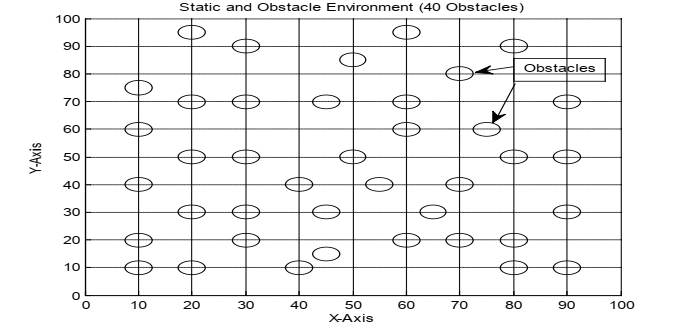
\includegraphics[width = 0.8\textwidth]{Caps/Figs/resultados/pista.png}
   \label{fig:pista-testes}
    \fonte{\cite{memon2015autonomous}}
\end{figure}

Espera-se que o robô consiga desviar de obstáculos de maneira seletiva e mesmo que o ambiente sofra alterações dinâmicas, ainda será possível encontrar uma rota viável. Alterando-se a posição dos objetos dinamicamente o robô conseguirá diferenciar obstáculos de não obstáculos.

O algoritmo de visão computacional será implementado e avaliado sua acurácia para detectar obstáculos em tempo real, durante a movimentação do RMA. O algoritmo de controle desempenhará o papel de planejar as novas trajetórias para a movimentação.

O RMA será prototipado utilizando um Raspberry Pi e um Arduino, onde serão integrados os sensores e atuadores. Este contará com um chassi visto na Figura~\ref{fig:chassi}, motores, rodas, sensores de imagem e ultrassônicos. A programação será realizada em C para o Arduino, pela Arduino IDE, onde será definido sua lógica de movimentação; e em Python para o Raspberry Pi que irá tratar a detecção dos objetos.

Os sensores ultrassônicos atuarão como última ação do RMA, caso o sistema de visão computacional ou o controle de sua trajetória falhe.

\begin{figure}[!hbtp]
  \centering
   \caption{Chassi.}
    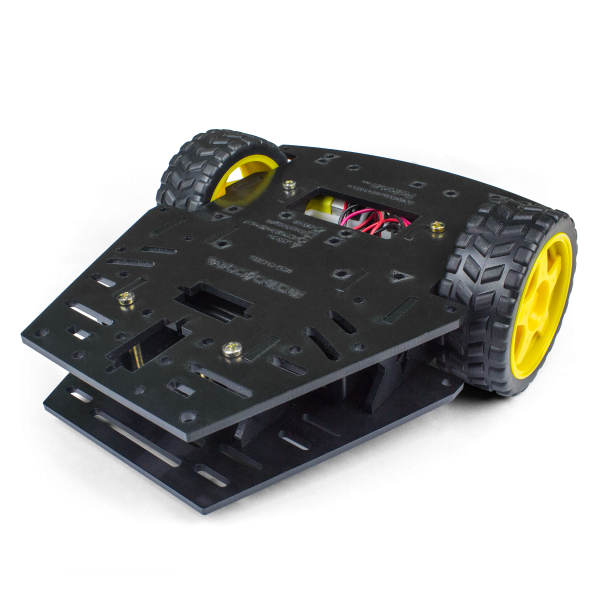
\includegraphics[width = 0.8\textwidth]{Caps/Figs/resultados/582_1_H.png}
   \label{fig:chassi}
    \fonte{Robocore}
\end{figure}